\documentclass[xcolor=dvipsnames]{beamer}

\usetheme{AnnArbor}
\usepackage{dsfont}
\usepackage{amsmath}
\usepackage{caption}
\usepackage{hyperref}
\usepackage{xcolor}
\usepackage{color}
\usepackage{commath}
\usepackage{physics}
\usepackage{enumerate}
\usepackage{hyperref}
\usepackage{graphics}
\usepackage{graphicx}
\usepackage{subcaption}

%\usepackage[backend=bibtex, style=authoryear-comp]{biblatex}

\setbeamertemplate{bibliography item}{\insertbiblabel}
\beamertemplatenavigationsymbolsempty

\usepackage{filecontents}
\begin{filecontents}{\jobname.bib}
\end{filecontents}
\usepackage[style=authoryear]{biblatex}
\renewcommand*{\nameyeardelim}{\addcomma\addspace}
\addbibresource{\jobname.bib}

\newcommand{\customcite}[1]{\citeauthor{#1} (\citeyear{#1})}

\newtheorem{satz}{Satz}

\setbeamertemplate{footline}[page number]

\usecolortheme{seagull}
\setbeamercolor{frametitle}{fg=blue,bg=White}

%\DeclareMathOperator*{\argmax}{arg\, max}
%\DeclareMathOperator*{\argmin}{arg\, min}
%\setbeamertemplate{section in toc}[sections numbered]
%\setbeamertemplate{subsection in toc}[subsections numbered]
%\AtBeginSection[]
%{
%\begin{frame}
%\frametitle{Überblick}
%\tableofcontents[currentsection]
%\end{frame}
%}
%
%\AtBeginSubsection[
% {\frame<beamer>{\frametitle{Überblick}   
%  \tableofcontents[currentsection,currentsubsection]}}%
%]%
%{
 % \frame<beamer>{ 
 %   \frametitle{Überblick}   
   % \tableofcontents[currentsection,currentsubsection]}
%}

\title{Twitter in the Parliament - A Text-based Analysis of German Political Entities}
%\author{Patrick Schulze}
\date{7. Juli 2020}
\author[author1]{Patrick Schulze, Simon Wiegrebe\\[10mm]{\small Supervisors:\\ Prof. Dr. Christian Heumann, Prof. Dr. Paul W. Thurner}}

\begin{document}

\begin{frame}
\titlepage
\end{frame}

%\begin{frame}
%\frametitle{Überblick}
%\tableofcontents[]
%\end{frame}

\begin{frame}
\frametitle{Covariate-level Topic Analysis}
\framesubtitle{Overview}
\begin{itemize}
\item Explore estimated topical structure with respect to different dimensions, e.g.\ membership in political party, time, $\dots$
\item Precisely: examine relationship between document-level prevalence covariates $\boldsymbol{x}_d$ and topic proportions $\boldsymbol{\theta}_d$
\item Natural idea: regress topic proportions on prevalence covariates
\begin{itemize}
\item In standard regression analysis, dependent variable is realization of random variable
\item In STM, however, we have access to posterior of topic proportions $\boldsymbol{\theta}_d$
\item If we "na{\"i}vely" use mean/mode of this posterior as dependent variable of regression, much information is lost
\item Solution: perform sampling technique known as "method of composition" in social sciences
\end{itemize}
\item Alternatively: direct assessment of logistic normal distribution with estimated topical prevalence parameters $\hat{\boldsymbol{\Gamma}}$ and $\hat{\boldsymbol{\Sigma}}$
\end{itemize}
\end{frame}

\begin{frame}
\frametitle{Covariate-level Topic Analysis}
\framesubtitle{Method of Composition: Usage within R Package \textit{stm}}
\begin{itemize}
\item Let $\boldsymbol{\theta}_{(k)}:=(\theta_{1,k}, \dots, \theta_{D,k})^T \in [0,1]^{D}$ denote proportion of $k$-th topic for all $D$ documents
\item Method of Composition (repeat $m$ times):
\begin{enumerate}
\item Sample $\boldsymbol{\theta}^*_{(k)}$ from (variational) posterior of $\boldsymbol{\theta}_{(k)}$ estimated by STM
\item Run regression model with response $\boldsymbol{\theta}^*_{(k)}$ and covariates $\boldsymbol{X}$ to obtain estimates of regression coefficients $\hat{\boldsymbol{\xi}}^*$ and covariance of $\hat{\boldsymbol{\xi}}^*$, $\hat{\boldsymbol{V}}^*_{\xi}$.
\item Sample $\tilde{\boldsymbol{\xi}}^*$ from $F(\hat{\boldsymbol{\xi}}^*, \hat{\boldsymbol{V}}^*_{\xi})$, where $F$ is asymptotic distribution of $\hat{\boldsymbol{\xi}}^*$.
\end{enumerate}
\item Idea: samples $\tilde{\boldsymbol{\xi}}^*$ take into account uncertainty in $\boldsymbol{\theta}_{(k)}$
\item Visualization of topic-metadata relationship: For observation $\boldsymbol{x}_{\text{pred}}$, plot $\boldsymbol{x}_{\text{pred}}$ vs. predicted response with $\boldsymbol{x}_{\text{pred}}^T \tilde{\boldsymbol{\xi}}^*$ as linear predictor
\end{itemize}
\end{frame}

\begin{frame}
\frametitle{Covariate-level Topic Analysis}
\framesubtitle{Method of Composition: Usage within R Package \textit{stm}}
\begin{enumerate}
\item In STM, regression model in step 2 is OLS; however OLS not appropriate to model proportions
\item Mixing of Bayesian and frequentist approach questionable! From Bayesian perspective $\tilde{\boldsymbol{\xi}}^*$ can only be considered sample from posterior of $\boldsymbol{\xi}$ in certain bayesian regression models with questionable (uniform) prior assumptions.
\item Using $\boldsymbol{x}_{\text{pred}}^T \tilde{\boldsymbol{\xi}}^*$  as linear predictor does \textit{not} yield sample of posterior predictive distribution
\item Separate modeling of topic proportions neglects dependence among variables
\end{enumerate}
\end{frame}

\begin{frame}
\frametitle{Covariate-level Topic Analysis}
\framesubtitle{Method of Composition: Usage within R Package \textit{stm}}
\begin{itemize}
\item Notation:
\begin{itemize}
\item $\boldsymbol{\theta}_{(k)}:=(\theta_{1,k}, \dots, \theta_{D,k})^T \in [0,1]^{D}$: proportion of $k$-th topic for all $D$ documents
\item $q(\boldsymbol{\theta}_{(k)} | \boldsymbol{X}, \boldsymbol{W})$: approximate variational posterior of $\boldsymbol{\theta}_{(k)}$
\item $q(\hat{\boldsymbol{\xi}} | \boldsymbol{X}, \boldsymbol{\theta}_{(k)})$: (normal) distribution of estimated regression coefficients $\hat{\boldsymbol{\xi}}$ from OLS regression $\boldsymbol{\theta}_{(k)} = \boldsymbol{X}\boldsymbol{\xi} + \boldsymbol{\epsilon}$, where $\boldsymbol{\epsilon} \sim \mathcal{N}(0,\sigma^2\boldsymbol{I})$
\end{itemize}
\item Method of composition:
\begin{enumerate}[{1)}]
\item Draw $\boldsymbol{\theta}_{(k)}^* \sim q(\boldsymbol{\theta}_{(k)} | \boldsymbol{X}, \boldsymbol{W})$.
\item Draw $\hat{\boldsymbol{\xi}}^* \sim q(\hat{\boldsymbol{\xi}} | \boldsymbol{X}, \boldsymbol{\theta}_{(k)}^*)$.
\end{enumerate}
\item It then holds that $\hat{\boldsymbol{\xi}}_1^*, \dots, \hat{\boldsymbol{\xi}}_m^*$ is an i.i.d.\ sample from the marginal posterior of regression coefficients
\begin{align*}
q(\boldsymbol{\xi} | \boldsymbol{X}, \boldsymbol{W}) = \int_{\boldsymbol{\theta}_{(k)}} q(\boldsymbol{\xi} | \boldsymbol{X}, \boldsymbol{\theta}_{(k)}) q(\boldsymbol{\theta}_{(k)} | \boldsymbol{X}, \boldsymbol{W}) \text{d} \boldsymbol{\theta}_{(k)} 
\end{align*}
\end{itemize}
\end{frame}

\begin{frame}
\begin{itemize}
\item Problem: OLS regression not suitable for (sampled) proportions, which are restricted to interval (0,1)
\item[$\Rightarrow$] Estimated relationship between proportions and prevalence covariates might involve negative estimated proportions
\end{itemize}
\frametitle{Covariate-level Topic Analysis}
\framesubtitle{Method of Composition: Usage within R Package \textit{stm}}
  \begin{figure}[h!]
  \centering
  \captionsetup{justification=centering,margin=2cm}
  \begin{subfigure}[b]{0.4\linewidth}
    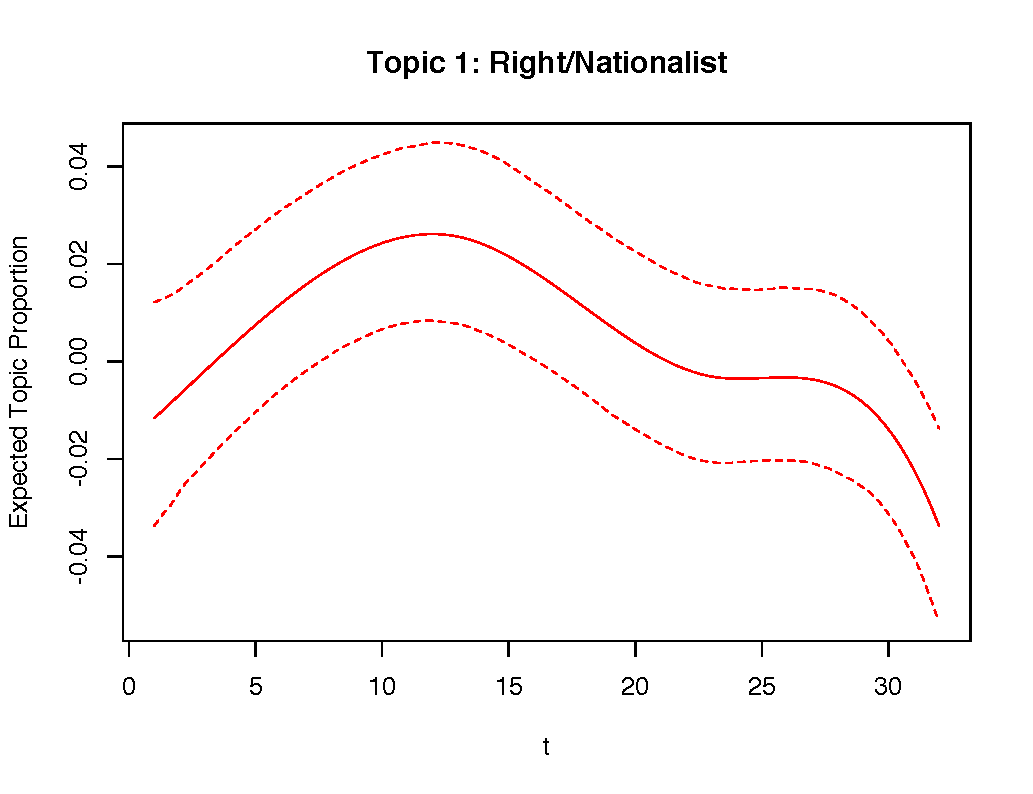
\includegraphics[width=\linewidth]{../../plots/presentation/estEffect_topic1.pdf}
  \end{subfigure}
  \begin{subfigure}[b]{0.4\linewidth}
    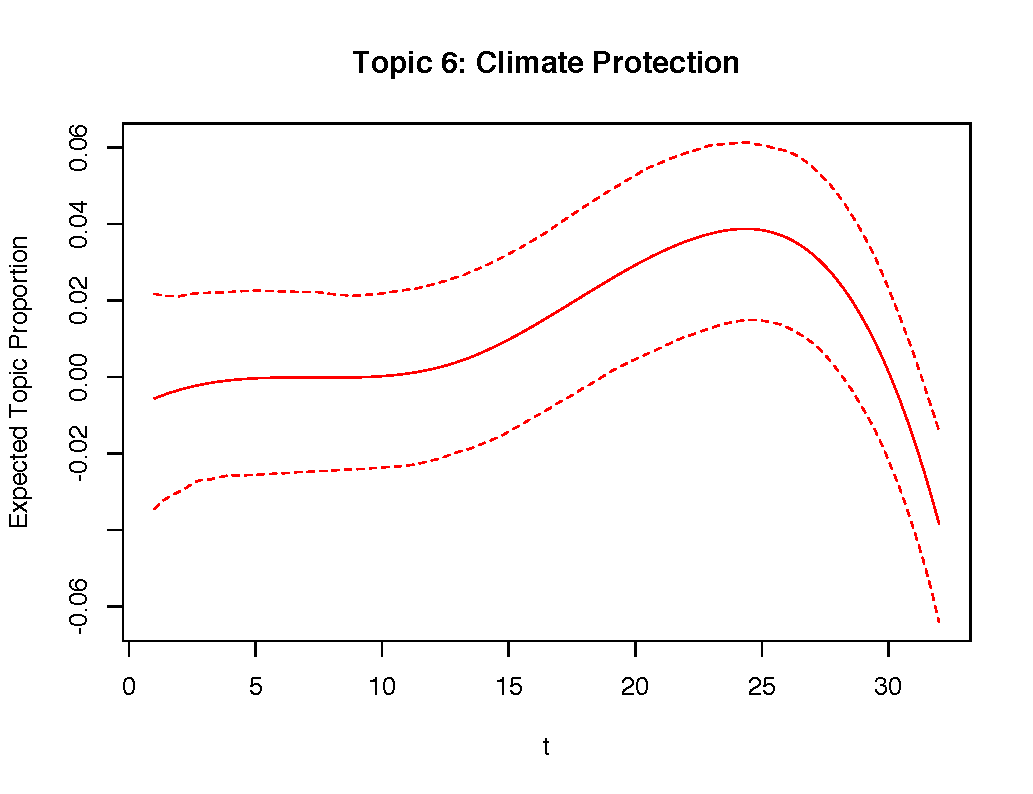
\includegraphics[width=\linewidth]{../../plots/presentation/estEffect_topic6.pdf}
  \end{subfigure}
  \caption{Emprical mean and 95\% credible intervals for topics 1 and 6 over time, estimated using \textit{estimateEffect} from the \textit{stm} package.}
  \label{fig:estEffect_topic16}
\end{figure}
\end{frame}

\begin{frame}
\frametitle{Covariate-level Topic Analysis}
\framesubtitle{Method of Composition: Extension of existing approach}
\begin{itemize}
\item Instead of OLS regression, we can use a beta regression or a quasibinomial GLM (both with logit-link) to adequately model proportions
\item In this case, regression coefficients are \textit{asymptotically} normally distributed
\end{itemize}
\begin{figure}[h!]
  \centering
  \captionsetup{justification=centering,margin=2cm}
  \begin{subfigure}[b]{0.4\linewidth}
    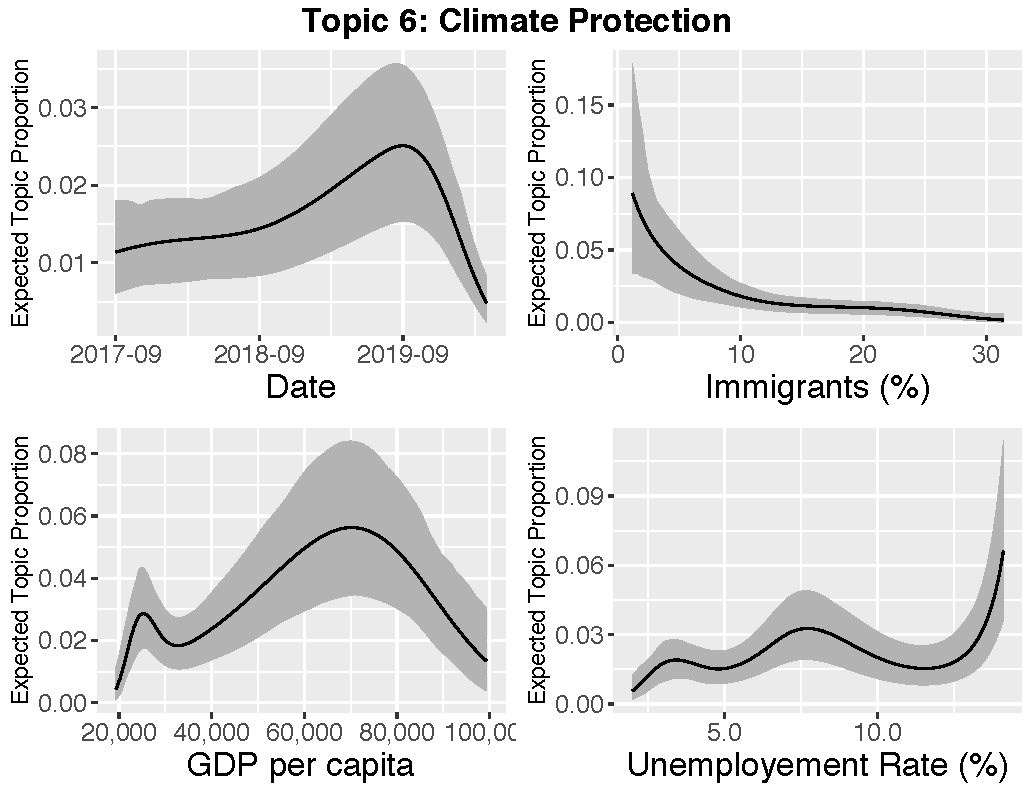
\includegraphics[width=\linewidth]{../../plots/presentation/quasi_t6_cont.pdf}
  \end{subfigure}
  \begin{subfigure}[b]{0.4\linewidth}
    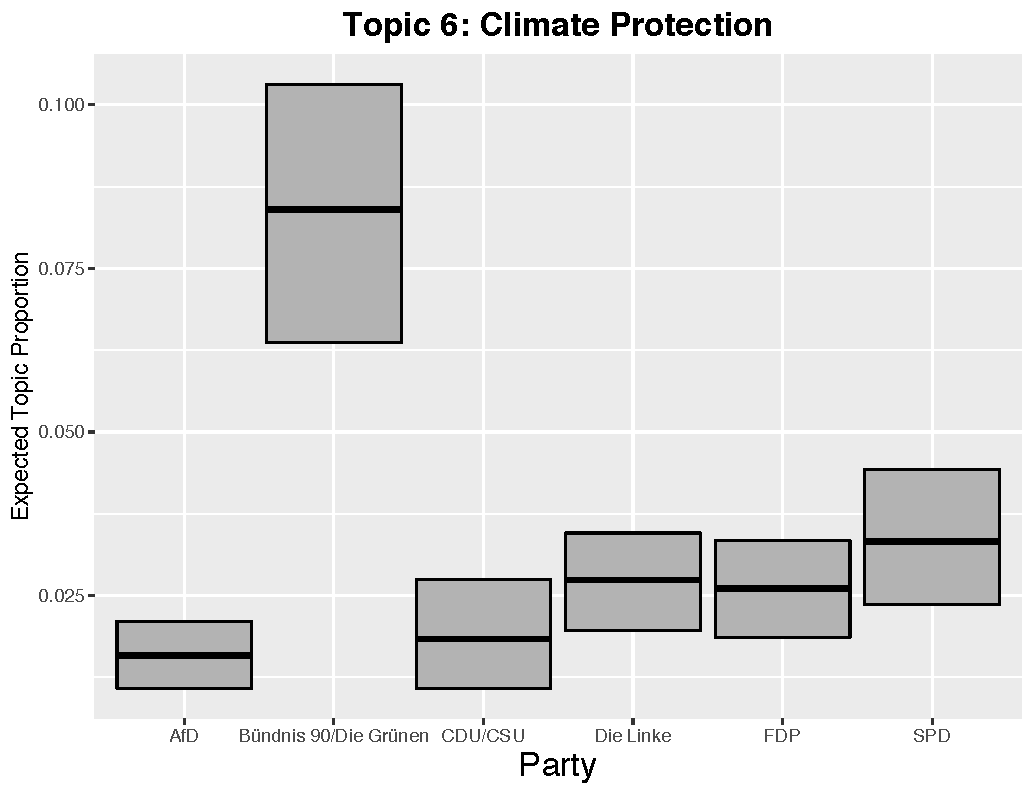
\includegraphics[width=\linewidth]{../../plots/presentation/quasi_t6_cat.pdf}
  \end{subfigure}
  \caption{Empirical mean and 95\% credible intervals, obtained using a quasibinomial GLM.}
  \label{fig:quasi_t46_cont}
\end{figure}
\end{frame}

\begin{frame}
\frametitle{Covariate-level Topic Analysis}
\framesubtitle{Problem: Univariate Modeling of Proportions}
\begin{itemize}
\item Remember, by assumption: $\boldsymbol{\theta}_d \sim \text{LogisticNormal}(\boldsymbol{\Gamma}^T\boldsymbol{x}_d^T, \boldsymbol{\Sigma})$
\item Logistic normal distribution assumes high dependence among individual components
\item However, regression within method of composition uses \textit{univariate} k-th topic proportion as dependant variable 
\item Problem with this approach: dependence among components neglected $\Rightarrow$ especially uncertainty estimates are unrealistic
\end{itemize}
\end{frame}

\begin{frame}
\frametitle{Covariate-level Topic Analysis}
\framesubtitle{Multivariate Modeling via Logistic Normal Distribution}
\begin{itemize}
\item Inference within STM involves finding estimates $\hat{\boldsymbol{\Gamma}}$ and $\hat{\boldsymbol{\Sigma}}$
\item Idea: plug estimates into logistic normal distribution $\Rightarrow$ for a given covariate value $\boldsymbol{x}^*_d$, "predict" topic proportion as
$\boldsymbol{\theta}^*_d \sim \text{LogisticNormal}(\hat{\boldsymbol{\Gamma}}^T(\boldsymbol{x}_d^*)^T, \hat{\boldsymbol{\Sigma}})$
\item Ideally, we would apply fully Bayesian approach and sample from (variational) posterior of $\boldsymbol{\Gamma}$ (and update $\boldsymbol{\Sigma}$, which is obtained via MLE) $\Rightarrow$ "Predictive Posterior" of topic proportions
\item However, output obtained using R package \textit{stm} does not allow for simple implementation of such a procedure (i.e., sampling from variational posterior of $\boldsymbol{\Gamma}$ and updating $\boldsymbol{\Sigma}$); yet, possible in theory!
\end{itemize}
\end{frame}

\begin{frame}
\begin{itemize}
\item Still, our results suggest a high discrepancy between:
\begin{itemize}
\item Distribution of topic proportions assumed in generative process of STM
\item Impression we gain of this distribution via separate modeling of topics.
\end{itemize}
\item Fully Bayesian approach would most likely yield even higher uncertainty
\end{itemize}
\frametitle{Covariate-level Topic Analysis}
\framesubtitle{Multivariate Modeling via Logistic Normal Distribution}
\begin{figure}[h!]
  \centering
  \captionsetup{justification=centering}
  \begin{subfigure}[b]{0.4\linewidth}
    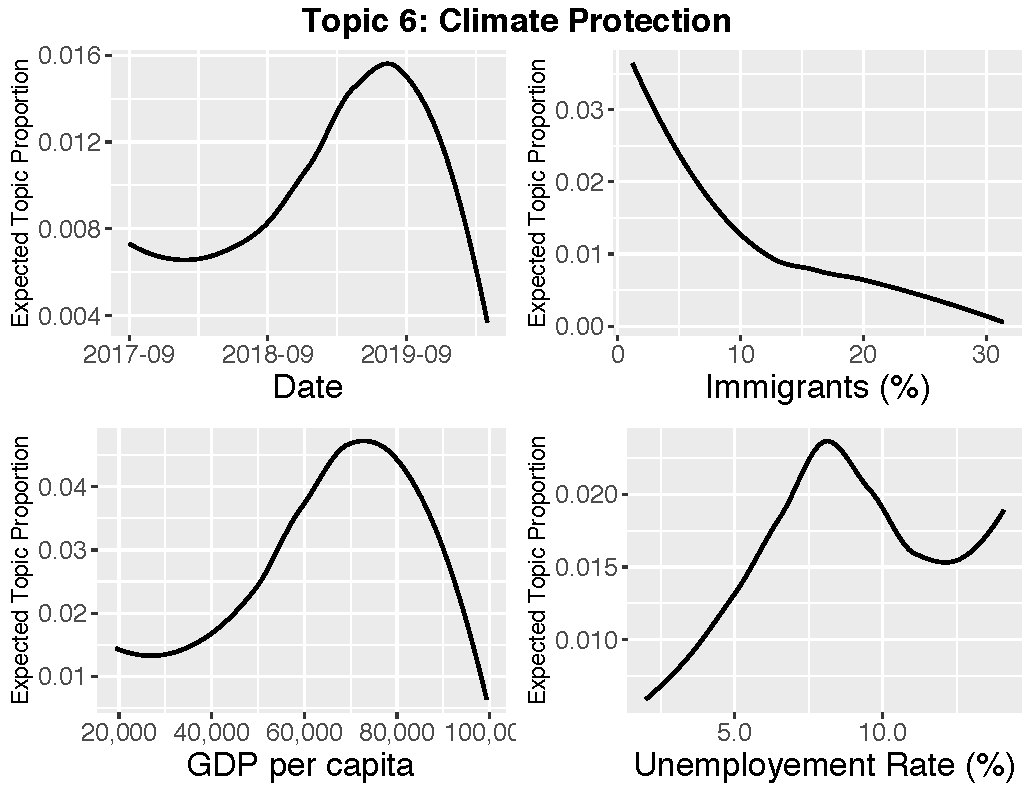
\includegraphics[width=\linewidth]{../../plots/presentation/direct_t6_without_credible.pdf}
  \end{subfigure}
  \begin{subfigure}[b]{0.4\linewidth}
    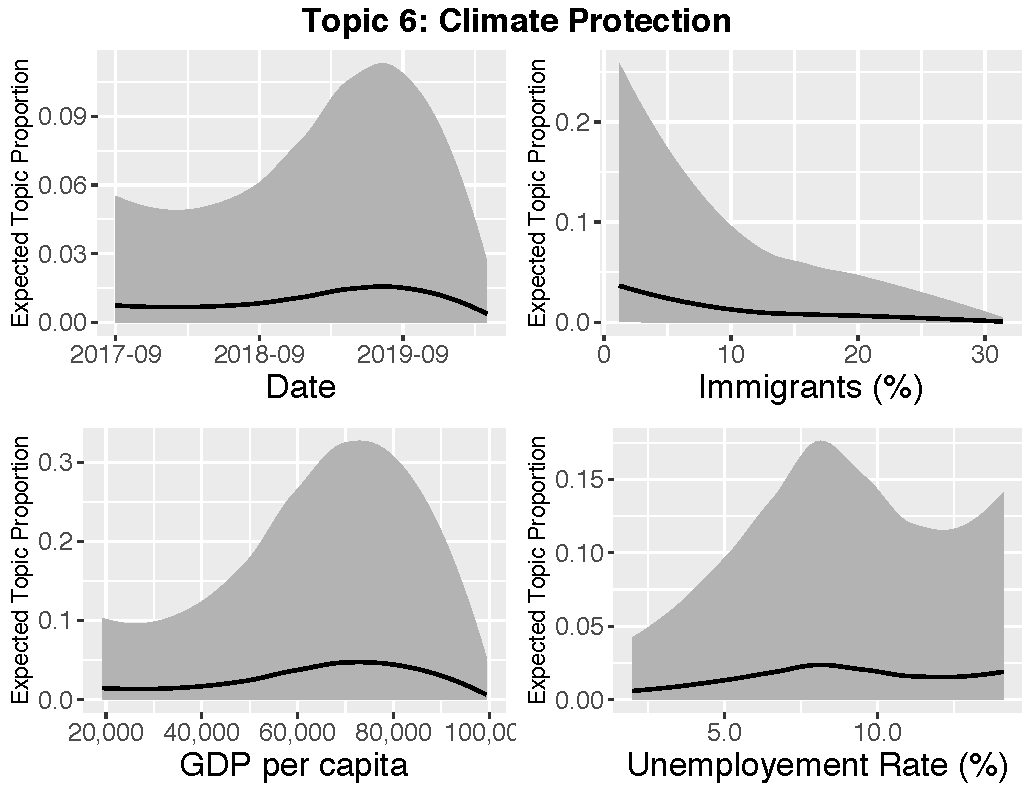
\includegraphics[width=\linewidth]{../../plots/presentation/direct_t6_with_credible.pdf}
  \end{subfigure}
  \caption{Smooth effects without credible intervals (left) and smooth effects with credible intervals (right)}
  \label{fig:directassessment}
\end{figure}
\end{frame}

\begin{frame}
\frametitle{Bibliography}
\printbibliography
\end{frame}
\end{document}